% !TeX program = pdflatex
% !TeX encoding = UTF-8
\documentclass[11pt,aspectratio=169,t]{beamer}
% Все презентации курса компилируются только pdflatex.
\usepackage{iftex}
\RequirePDFTeX
\usepackage{cmap}
\usepackage[T2A]{fontenc}
\usepackage[utf8]{inputenc}
\usepackage[english,russian]{babel}
\usepackage{PTSerif}
\usepackage{amsmath,amsfonts,amssymb}
\usepackage{graphicx,microtype,anyfontsize,tikz}
\usepackage{ragged2e}
\usetikzlibrary{arrows.meta,calc}

\usetheme{default}
\usefonttheme{serif}
\DeclareMathOperator{\sen}{sen}
\bibliographystyle{apalike}

% Общие сведения; номер лекции, её название и дата задаются в N.tex.
\newcommand{\coursename}{Введение в маневрирование КА}
\author{Чиняев Владимир Николаевич}
\institute{Московский физико-технический институт}

% Книжное оформление с голубым акцентом.
\definecolor{coursepaper}{HTML}{FBF9F3}
\definecolor{courseink}{HTML}{302B28}
\definecolor{courseaccent}{HTML}{187AA5}
\definecolor{coursemuted}{HTML}{6D6560}
\definecolor{courserule}{HTML}{A9CADA}
\definecolor{coursetint}{HTML}{EDF4F6}
\tikzset{
  course diagram/.style={font=\fontsize{9.5}{11.5}\selectfont,
    line cap=round,line join=round,>=Latex},
  orbit line/.style={draw=courseaccent,line width=1pt},
  aux line/.style={draw=courserule,line width=.5pt},
  vector line/.style={draw=courseink,line width=.65pt,->},
  angle line/.style={draw=courseaccent,line width=.8pt,->},
  orbit point/.style={circle,fill=courseaccent,inner sep=1.7pt}
}
\setbeamercolor{normal text}{fg=courseink,bg=coursepaper}
\setbeamercolor{background canvas}{bg=coursepaper}
\setbeamercolor{structure}{fg=courseaccent}
\setbeamercolor{alerted text}{fg=courseaccent}
\setbeamercolor{frametitle}{fg=courseink,bg=coursepaper}
\setbeamercolor{footline}{fg=coursemuted,bg=coursepaper}
\setbeamercolor{caption name}{fg=courseaccent}

% Основной текст — 11/14 pt; подписи к рисункам — 9.5/11.5 pt.
\let\coursenormalsize\normalsize
\renewcommand{\normalsize}{\coursenormalsize\fontsize{11}{14}\selectfont}
\setbeamerfont{normal text}{size*={11pt}{14pt}}
\setbeamerfont{frametitle}{size*={20pt}{23pt},series=\mdseries}
\setbeamerfont{title}{size*={27pt}{31pt},series=\mdseries}
\setbeamerfont{subtitle}{size*={12.8pt}{15pt},series=\mdseries}
\setbeamerfont{author}{size*={10.8pt}{13pt}}
\setbeamerfont{institute}{size*={9.2pt}{11pt}}
\setbeamerfont{date}{size*={9pt}{11pt}}
\setbeamerfont{footline}{size*={6.8pt}{8pt}}
\setbeamerfont{caption}{size*={9.5pt}{11.5pt}}
\setbeamerfont{itemize/enumerate body}{size*={11pt}{14pt}}
\setbeamerfont{itemize/enumerate subbody}{size*={11pt}{14pt}}
\setbeamerfont{itemize/enumerate subsubbody}{size*={11pt}{14pt}}
\AtBeginDocument{\normalsize}

\setbeamersize{text margin left=6mm,text margin right=6mm}
\setbeamertemplate{navigation symbols}{}
\setbeamertemplate{headline}{}
\setbeamertemplate{caption}[numbered]
\setbeamertemplate{itemize items}[circle]

% Стандартные блоки Beamer позволяют группировать текст и формулы.
\setbeamertemplate{blocks}[default]
\setbeamerfont{block title}{size*={11pt}{14pt},series=\bfseries}
\setbeamerfont{block body}{size*={11pt}{14pt}}
\setbeamercolor{block title}{fg=courseaccent,bg=coursepaper}
\setbeamercolor{block body}{fg=courseink,bg=coursetint}
\setbeamercolor{block title alerted}{parent=block title}
\setbeamercolor{block body alerted}{parent=block body}
\setbeamercolor{block title example}{parent=block title}
\setbeamercolor{block body example}{parent=block body}

% Компактный заголовок; его высота учитывается при размещении содержания.
\setbeamertemplate{frametitle}{%
  \vskip4.5mm%
  \begin{beamercolorbox}[wd=\textwidth,sep=0pt]{frametitle}
    \usebeamerfont{frametitle}\strut\insertframetitle\strut\par
    \vskip2mm%
    {\color{courseaccent}\hrule height .55pt}
  \end{beamercolorbox}%
}

% Нижний колонтитул: курс слева, лекция и номер слайда справа.
\setbeamertemplate{footline}{%
  \begin{beamercolorbox}[wd=\paperwidth,ht=5.5mm,dp=0pt]{footline}
    \begin{tikzpicture}[remember picture,overlay,x=1mm,y=1mm]
      \begin{scope}[shift={(current page.south west)}]
        \draw[courserule,line width=.3pt] (6,5.5)--(154,5.5);
        \node[text=coursemuted,anchor=west,inner sep=0pt,
          font=\usebeamerfont{footline}] at (6,2.8) {\coursename};
        \node[text=coursemuted,anchor=east,inner sep=0pt,
          font=\usebeamerfont{footline}] at (154,2.8)
          {Лекция \arabic{lecture}\quad\textbullet\quad\insertframenumber};
      \end{scope}
    \end{tikzpicture}%
  \end{beamercolorbox}%
}

% Титульник рассчитан на 16:9 (160 × 90 мм), без нижнего колонтитула.
\setbeamertemplate{title page}{%
  \begin{tikzpicture}[remember picture,overlay,x=1mm,y=1mm]
    \begin{scope}[shift={(current page.south west)}]
      \node[text=coursemuted,anchor=north,font=\usebeamerfont{institute}]
        at (80,82) {\insertinstitute};
      \draw[courseaccent,line width=.55pt] (71,71)--(89,71);
      \node[text=courseink,align=center,text width=125mm,
        font=\usebeamerfont{title}] at (80,53)
        {\hyphenpenalty=10000\coursename\par};
      \node[text=courseaccent,align=center,text width=145mm,font=\usebeamerfont{subtitle}]
        at (80,32) {Лекция \arabic{lecture}. \inserttitle};
      \node[text=courseink,font=\usebeamerfont{author}]
        at (80,19) {\insertauthor};
      \node[text=coursemuted,font=\usebeamerfont{date}]
        at (80,9) {\insertdate};
    \end{scope}
  \end{tikzpicture}%
}

\usepackage{booktabs,array,mathtools}
\setlength{\abovedisplayskip}{5pt}
\setlength{\belowdisplayskip}{5pt}
\setlength{\abovedisplayshortskip}{3pt}
\setlength{\belowdisplayshortskip}{4pt}
\newcommand{\eqcompact}{\fontsize{10}{12}\selectfont}
\newcommand{\figcaption}[1]{{\usebeamerfont{caption}\color{coursemuted}#1\par}}
\newcommand{\derivationmathspacing}{%
  \setlength{\abovedisplayskip}{2pt}%
  \setlength{\belowdisplayskip}{3pt}%
  \setlength{\abovedisplayshortskip}{2pt}%
  \setlength{\belowdisplayshortskip}{2pt}%
  \setlength{\jot}{2pt}}
\newcommand{\vect}[1]{\boldsymbol{#1}}
\newcommand{\norm}[1]{\left\lVert#1\right\rVert}
\newcommand{\dd}{\mathop{}\!\mathrm d}
\DeclareMathOperator{\diag}{diag}
\setcounter{lecture}{9}
\title{Манёвры уклонения от столкновения}
\date{17 ноября 2026 г.}
% Generated by avoidance_example.py
\newcommand{\ExamplePeriod}{5828{,}517}
\newcommand{\ExampleLead}{2331{,}407}
\newcommand{\ExampleNominalMiss}{29{,}155}
\newcommand{\ExampleNominalPc}{5{,}88\cdot10^{-3}}
\newcommand{\ExampleRelativeSpeed}{7{,}5842}
\newcommand{\ExampleOptimalDV}{0{,}097840}
\newcommand{\ExampleOptimalMiss}{348{,}632}
\newcommand{\ExampleOptimalNonlinearPc}{1{,}00\cdot10^{-5}}
\newcommand{\ExampleOptimalNonlinearMiss}{348{,}637}
\newcommand{\ExampleOptimalTCA}{0{,}026143}
\newcommand{\ExampleExecutionPc}{1{,}18\cdot10^{-5}}
\newcommand{\ExampleSafeDV}{0{,}100996}
\newcommand{\ExampleSafePc}{8{,}00\cdot10^{-6}}
\newcommand{\ExampleSafeNonlinearPc}{8{,}00\cdot10^{-6}}
\newcommand{\ExampleSafeNonlinearMiss}{360{,}573}
\newcommand{\ExampleSafeTCA}{0{,}026988}
\newcommand{\ExampleGRepeat}{1{,}22\cdot10^{-9}}
\newcommand{\ExamplePcRepeat}{6{,}60\cdot10^{-15}}
\newcommand{\ExampleMatrixG}{\begin{pmatrix}-483{,}069&-3321{,}815&0{,}000\\2882{,}996&4276{,}692&-256{,}984\end{pmatrix}}
\newcommand{\ExampleCovarianceMatrix}{\begin{pmatrix}14233{,}213&-18042{,}098\\-18042{,}098&27366{,}787\end{pmatrix}}


\begin{document}

\begin{frame}[plain]\titlepage\end{frame}

% Главы 1--3 методички collision-avoidance.tex.
\begin{frame}{Манёвр уклонения}
\relax\derivationmathspacing
Манёвр изменяет движение КА, снижая вероятность столкновения
при допустимом отклонении от рабочей орбиты.
\par\smallskip
\begin{columns}[T,onlytextwidth]
\begin{column}{.48\textwidth}
\textbf{Один импульс}
{\eqcompact\derivationmathspacing
\[
\begin{aligned}
\min_{\mathclap{t_m,\,\Delta\vect V\in\mathcal A(t_m)}}\quad
 &\norm{\Delta\vect V},\\[5pt]
\mathrm{s.t.}\quad
 &P_c(t_m,\Delta\vect V)\leqslant P_{\text{доп}},\\[4pt]
 &t_m\in[t_{m,\min},t_{m,\max}].
\end{aligned}
\]
\[
J=\norm{\Delta\vect V},\qquad
\vect y=(a,e,\omega,i,\Omega,M)^\top.
\]
}
Конечное состояние отдельно не предписывается.
\end{column}
\begin{column}{.49\textwidth}
\begin{itemize}
\setlength{\itemsep}{3pt}
\item $\mathrm{sc}$ (spacecraft) --- управляемый КА.
\item $\mathrm{obj}$ (object) --- опасный объект; в нашей модели не маневрирует.
\item $P_c$ --- вероятность за рассматриваемое сближение.
\item $\mathcal A(t_m)$ --- допустимые направления и величины импульса.
\item Порог $P_{\text{доп}}$ задан условиями задачи.
\end{itemize}
\end{column}
\end{columns}
\end{frame}

\begin{frame}{Данные и управление}
\relax\derivationmathspacing
\begin{columns}[T,onlytextwidth]
\begin{column}{.48\textwidth}
\textbf{Начальные состояния и ковариации}
\par\smallskip
Прогноз обоих объектов относится к одному времени и одной системе координат.
{\eqcompact\derivationmathspacing
\[
\vect R_{\mathrm{sc}}^+=\vect R_{\mathrm{sc}}^-,\qquad
\vect V_{\mathrm{sc}}^+=\vect V_{\mathrm{sc}}^-+
\Delta\vect V_{\text{ИСК}},
\]
\[
\Delta\vect V=
\begin{pmatrix}\Delta V_r&\Delta V_t&\Delta V_n\end{pmatrix}^{\!\top},
\]
\[
\Delta\vect V_{\text{ИСК}}=
\begin{bmatrix}\vect e_r&\vect e_t&\vect e_n\end{bmatrix}\Delta\vect V.
\]
}
Импульс приложен в $t_m$; базис --- предманёвренная ОСК.
После скачка скорости определяется новая орбита.
\end{column}
\begin{column}{.49\textwidth}
\textbf{Предварительный отбор пар}
\begin{enumerate}
\setlength{\itemsep}{2pt}
\item Сравнить кеплеровы диапазоны
{\eqcompact\[
\bigl[a(1-e),\,a(1+e)\bigr]
\]}
с запасом на размеры и ошибки.
\item Исключить непересекающиеся диапазоны при принятом запасе.
\item Для остальных пар прогнозом уточнить время и расстояние сближения.
\end{enumerate}
Близость орбит не гарантирует сближения.
\end{column}
\end{columns}
\end{frame}

\begin{frame}{Относительное движение}
\relax\derivationmathspacing
Номинальные траектории --- ожидаемые состояния без случайных ошибок.
\par\smallskip
\begin{columns}[T,onlytextwidth]
\begin{column}{.48\textwidth}
\textbf{В инерциальных осях}
{\eqcompact\derivationmathspacing
\[
\begin{aligned}
\vect\rho&=\vect R_{\mathrm{obj}}-\vect R_{\mathrm{sc}},\\
\vect v_{\mathrm{rel}}&=\vect V_{\mathrm{obj}}-\vect V_{\mathrm{sc}},\\
\dot{\vect\rho}&=\vect v_{\mathrm{rel}}.
\end{aligned}
\]
}
$t_{\mathrm{ca}}$ --- момент наибольшего сближения (TCA, time of closest approach).
{\eqcompact\derivationmathspacing
\[
d_{\min}=\norm{\vect\rho(t_{\mathrm{ca}})}.
\]
}
В ОСК производная координат учитывает вращение базиса.
\end{column}
\begin{column}{.49\textwidth}
\centering
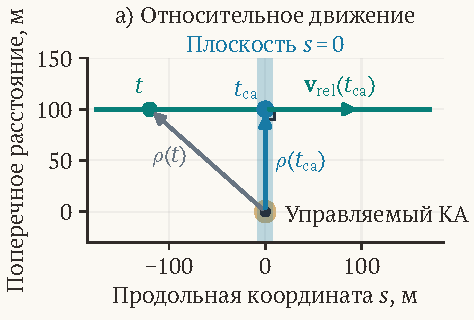
\includegraphics[width=\linewidth,height=41mm,keepaspectratio]{images/concept-geometry-a-slide.pdf}\par
\figcaption{В TCA относительные положение и скорость перпендикулярны.}
\end{column}
\end{columns}
\end{frame}

\begin{frame}{Момент наибольшего сближения}
\relax\derivationmathspacing
\begin{columns}[T,onlytextwidth]
\begin{column}{.48\textwidth}
\textbf{Первая производная}
{\eqcompact\derivationmathspacing
\[
\frac{\dd}{\dd t}\frac{\norm{\vect\rho}^2}{2}
=\frac{\dot{\vect\rho}^{\top}\vect\rho+
\vect\rho^\top\dot{\vect\rho}}{2}
\]
\[
=\vect\rho^\top\vect v_{\mathrm{rel}}.
\]
\[
\boxed{\vect\rho^\top\vect v_{\mathrm{rel}}=0.}
\]
}
Условие стационарности квадрата расстояния задаёт кандидата на TCA.
\par\smallskip
Несколько локальных минимумов на интервале оцениваются отдельно.
\end{column}
\begin{column}{.49\textwidth}
\textbf{Проверка локального минимума}
{\eqcompact\derivationmathspacing
\[
\vect a_{\mathrm{sc}}=\dot{\vect V}_{\mathrm{sc}},\qquad
\vect a_{\mathrm{obj}}=\dot{\vect V}_{\mathrm{obj}},
\]
\[
\vect a_{\mathrm{rel}}=\vect a_{\mathrm{obj}}-\vect a_{\mathrm{sc}}.
\]
\[
\begin{aligned}
\frac{\dd^2}{\dd t^2}\frac{\norm{\vect\rho}^2}{2}
&=\dot{\vect\rho}^{\top}\vect v_{\mathrm{rel}}
 +\vect\rho^\top\dot{\vect v}_{\mathrm{rel}}\\
&=\norm{\vect v_{\mathrm{rel}}}^2
 +\vect\rho^\top\vect a_{\mathrm{rel}}>0.
\end{aligned}
\]
}
$\vect a_{\mathrm{sc}},\vect a_{\mathrm{obj}}$ --- векторные ускорения;
$a$ --- скалярная большая полуось.
\end{column}
\end{columns}
\end{frame}

\begin{frame}{Локальная оценка времени}
\relax\derivationmathspacing
\begin{columns}[T,onlytextwidth]
\begin{column}{.48\textwidth}
\textbf{Разложение около эпохи $t$}
{\eqcompact\derivationmathspacing
\[
\begin{aligned}
\vect\rho(t+\tau)={}&\vect\rho(t)+\vect v_{\mathrm{rel}}(t)\tau\\
&+\tfrac12\vect a_{\mathrm{rel}}(t)\tau^2+O(\tau^3).
\end{aligned}
\]
\[
\vect\rho(t+\tau)\approx\vect\rho(t)+\vect v_{\mathrm{rel}}(t)\tau.
\]
}
Короткий пролёт: изменение относительной скорости за время $\tau$ мало.
\par\smallskip
Векторы в правой колонке вычислены в эпоху $t$.
\end{column}
\begin{column}{.49\textwidth}
\textbf{Минимум в прямолинейной модели}
{\eqcompact\derivationmathspacing
\[
\begin{aligned}
\norm{\vect\rho+\vect v_{\mathrm{rel}}\tau}^2
={}&\norm{\vect\rho}^2+2\tau\vect\rho^\top\vect v_{\mathrm{rel}}\\
&+\tau^2\norm{\vect v_{\mathrm{rel}}}^2,
\end{aligned}
\]
\[
\vect\rho^\top\vect v_{\mathrm{rel}}
 +\tau\norm{\vect v_{\mathrm{rel}}}^2=0,
\]
\[
\boxed{t_{\mathrm{ca}}-t\approx
-\frac{\vect\rho(t)^\top\vect v_{\mathrm{rel}}(t)}
 {\norm{\vect v_{\mathrm{rel}}(t)}^2}.}
\]
}
Знак поправки показывает, впереди или позади выбранной эпохи находится минимум.
\end{column}
\end{columns}
\smallskip
После манёвра относительные положение и скорость меняются: TCA определяется заново.
\end{frame}

\begin{frame}{Плоскость сближения}
\relax\derivationmathspacing
\begin{columns}[T,onlytextwidth]
\begin{column}{.48\textwidth}
{\eqcompact\derivationmathspacing
\[
\vect e_v=\frac{\vect v_{\mathrm{rel}}}{\norm{\vect v_{\mathrm{rel}}}},\qquad
\vect e_1,\vect e_2\perp\vect e_v,
\]
\[
P=\begin{bmatrix}\vect e_1^\top\\\vect e_2^\top\end{bmatrix},\qquad
PP^\top=I_2,
\]
\[
P^\top P=I_3-\vect e_v\vect e_v^\top,\qquad
\boxed{\vect b=P\vect\rho.}
\]
}
$\vect e_1,\vect e_2$ --- ортонормированные оси плоскости.
{\eqcompact\derivationmathspacing
\[
P\vect v_{\mathrm{rel}}=0,\qquad
\norm{\vect b(t_{\mathrm{ca}})}=d_{\min}.
\]
}
В прямолинейной модели продольное движение меняет время пролёта;
поперечное --- промах.
\end{column}
\begin{column}{.49\textwidth}
\centering
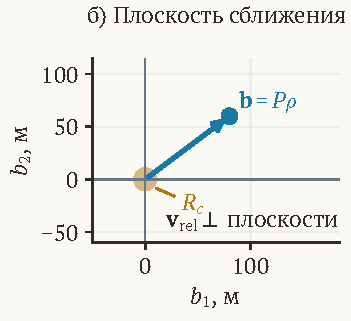
\includegraphics[width=\linewidth,height=44mm,keepaspectratio]{images/concept-geometry-b-slide.pdf}\par
\figcaption{Две координаты промаха в плоскости, перпендикулярной относительной скорости.}
\end{column}
\end{columns}
\end{frame}

\begin{frame}{Короткое сближение}
\relax\derivationmathspacing
\begin{columns}[T,onlytextwidth]
\begin{column}{.48\textwidth}
\textbf{Геометрическая область столкновения}
\par\smallskip
Каждый объект заменяется охватывающей его сферой.
{\eqcompact\derivationmathspacing
\[
R_c=R_{c,\mathrm{sc}}+R_{c,\mathrm{obj}},\qquad
\norm{\vect b}\leqslant R_c.
\]
}
Один объект рассматривается как точка, другой --- как сфера суммарного радиуса.
\par\smallskip
При неопределённом положении требуется вероятность попадания в круг столкновения.
\end{column}
\begin{column}{.49\textwidth}
\textbf{Условия прямолинейной модели}
\begin{itemize}
\setlength{\itemsep}{3pt}
\item Относительная траектория почти прямая.
\item Ковариация положения почти постоянна.
\item Неопределённость скорости мало меняет геометрию за пролёт.
\end{itemize}
{\eqcompact\derivationmathspacing
\[
\text{Продолжительность пролёта}\sim
\frac{L}{\norm{\vect v_{\mathrm{rel}}}}.
\]
}
$L$ --- существенный размер области неопределённости вдоль движения.
\end{column}
\end{columns}
\end{frame}

\begin{frame}{Неопределённость положения}
\relax\derivationmathspacing
\begin{columns}[T,onlytextwidth]
\begin{column}{.48\textwidth}
\textbf{Ошибки инерциального положения}
{\eqcompact\derivationmathspacing
\[
\mathbb{E}[\delta\vect R_{\mathrm{sc}}]=
\mathbb{E}[\delta\vect R_{\mathrm{obj}}]=0,
\]
\[
C_{\mathrm{sc}}=\mathbb{E}
 [\delta\vect R_{\mathrm{sc}}\delta\vect R_{\mathrm{sc}}^\top].
\]
}
Диагональные элементы --- дисперсии координат;
внедиагональные --- связи ошибок координат.
\par\smallskip
Собственные векторы задают главные направления эллипсоида,
корни собственных значений --- среднеквадратические ошибки.
\end{column}
\begin{column}{.49\textwidth}
\textbf{Относительная ошибка}
{\eqcompact\derivationmathspacing
\[
\delta\vect\rho=
\delta\vect R_{\mathrm{obj}}-\delta\vect R_{\mathrm{sc}},
\]
\[
\boxed{C_\rho=C_{\mathrm{sc}}+C_{\mathrm{obj}}}
\quad\text{при независимости},
\]
\[
\begin{aligned}
C_\rho={}&C_{\mathrm{sc}}+C_{\mathrm{obj}}\\
&-C_{\mathrm{sc},\mathrm{obj}}-C_{\mathrm{sc},\mathrm{obj}}^\top,
\end{aligned}
\]
\[
C_{\mathrm{sc},\mathrm{obj}}=
\mathbb{E}[\delta\vect R_{\mathrm{sc}}\delta\vect R_{\mathrm{obj}}^\top].
\]
\[
\boxed{C_b=PC_\rho P^\top\in\mathbb R^{2\times2}.}
\]
}
Далее ошибки определения состояний объектов независимы.
\end{column}
\end{columns}
\end{frame}

\begin{frame}{Перенос ковариации}
\relax\derivationmathspacing
Матрицы сопоставляются в одной эпохе, системе координат и единицах.
\par\smallskip
\begin{columns}[T,onlytextwidth]
\begin{column}{.48\textwidth}
\textbf{Перенос во времени}
{\eqcompact\derivationmathspacing
\[
\delta\vect y(t)=\Phi(t,t_i)\delta\vect y(t_i),
\]
\[
\boxed{C_y(t)=\Phi(t,t_i)C_y(t_i)\Phi^\top(t,t_i).}
\]
\[
\vect y=(a,e,\omega,i,\Omega,M)^\top.
\]
}
$C_y$ --- ковариация всех шести элементов; ошибками модели движения пренебрегаем.
\par\smallskip
Неопределённость большой полуоси приводит к росту ошибки фазы при увеличении времени прогноза.
\end{column}
\begin{column}{.49\textwidth}
\textbf{Переход к инерциальному положению}
{\eqcompact\derivationmathspacing
\[
C_k(t)=\frac{\partial\vect R_k}{\partial\vect y_k}
C_y(t)\left(\frac{\partial\vect R_k}{\partial\vect y_k}\right)^\top.
\]
}
Перенос выполняется отдельно для $k\in\{\mathrm{sc},\mathrm{obj}\}$.
\par\smallskip
Для ковариации в другом ортонормированном базисе:
{\eqcompact\derivationmathspacing
\[
C_{\text{ИСК}}=QCQ^\top.
\]
}
Столбцы $Q$ --- оси исходного базиса в инерциальных координатах.
\end{column}
\end{columns}
\end{frame}

\begin{frame}{Вероятность за короткий пролёт}
\relax\derivationmathspacing
\centering
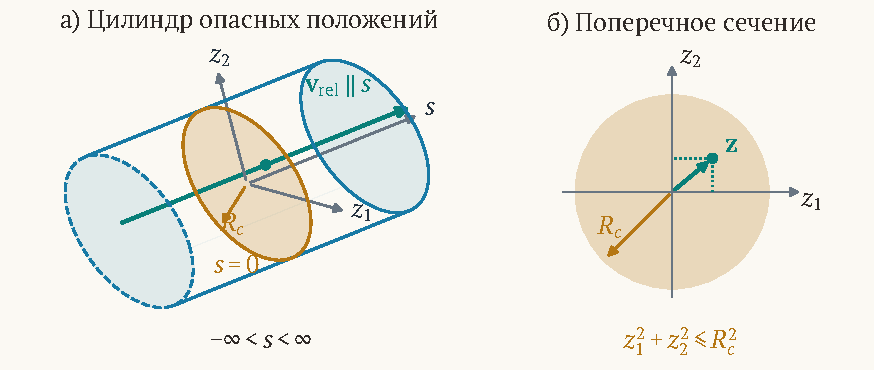
\includegraphics[width=\textwidth,height=40mm,keepaspectratio]{images/concept-cylinder-slide.pdf}
\par
{\eqcompact\derivationmathspacing
\[
P_c=\iint_{\norm{\vect z}\leqslant R_c}
\left(\int_{-\infty}^{\infty}p_3(\vect z,s)\,\dd s\right)
\dd z_1\dd z_2.
\]
}
\figcaption{$p_3$ --- трёхмерная плотность относительного положения;
$s$ --- координата вдоль скорости.
Интеграл по $s$ даёт поперечную плотность; независимость ошибок не требуется.}
\end{frame}

\begin{frame}{Вероятность столкновения}
\relax\derivationmathspacing
Гауссова проекция: математическое ожидание $\vect b$, ковариация $C_b$.
{\eqcompact\derivationmathspacing
\[
\boxed{P_c=\frac{1}{2\pi\sqrt{\det C_b}}
\iint_{\norm{\vect z}\leqslant R_c}
\exp\!\left[-\frac12(\vect z-\vect b)^\top C_b^{-1}(\vect z-\vect b)\right]
\dd z_1\dd z_2.}
\]
}
\begin{columns}[T,onlytextwidth]
\begin{column}{.48\textwidth}
\textbf{Что интегрируется}
\par\smallskip
Круг столкновения расположен в начале координат;
центр плотности --- в точке $\vect b$.
\par\smallskip
$P_c$ относится ко всему короткому пролёту.
Вероятность нахождения внутри сферы в один фиксированный момент --- другая величина.
\end{column}
\begin{column}{.49\textwidth}
\textbf{Контуры плотности}
{\eqcompact\derivationmathspacing
\[
(\vect z-\vect b)^\top C_b^{-1}(\vect z-\vect b)=k^2,
\]
\[
\text{Собственные значения }C_b:\ \sigma_1^2,\sigma_2^2,
\]
\[
\text{Полуоси: }k\sigma_1,\ k\sigma_2;\quad
\text{доля: }1-e^{-k^2/2}.
\]
}
При $k=1$ внутри эллипса около $39{,}3\%$ вероятности.
\end{column}
\end{columns}
\end{frame}

\begin{frame}{Главные оси ковариации}
\relax\derivationmathspacing
\centering
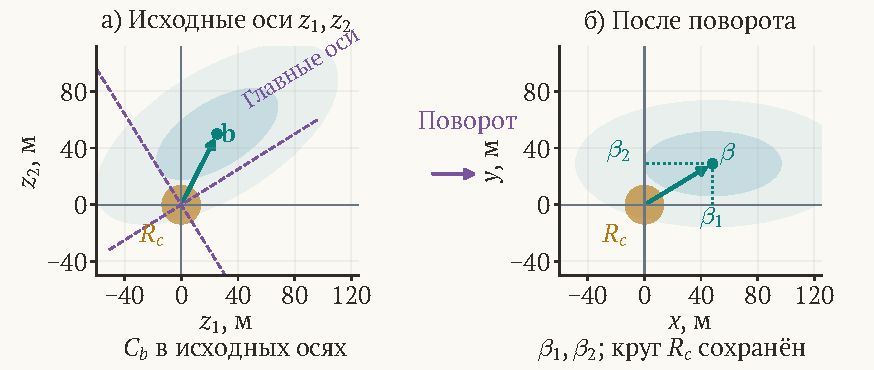
\includegraphics[width=\textwidth,height=42mm,keepaspectratio]{images/concept-principal-axes-slide.pdf}
\par
{\eqcompact\derivationmathspacing
\[
C_b\ \longrightarrow\ \diag(\sigma_1^2,\sigma_2^2).
\]
}
\figcaption{$\beta_1,\beta_2$ --- компоненты среднего вектора промаха в главных осях ковариации.
Поворот сохраняет круг столкновения.}
\end{frame}

\begin{frame}{Вычисление вероятности}
\relax\derivationmathspacing
В главных осях интегрируем по второй координате аналитически:
{\eqcompact\derivationmathspacing
\[
\begin{aligned}
P_c={}&\frac{1}{2\pi\sigma_1\sigma_2}
\int_{-R_c}^{R_c}e^{-(x-\beta_1)^2/(2\sigma_1^2)}
\left[\int_{-\sqrt{R_c^2-x^2}}^{\sqrt{R_c^2-x^2}}
e^{-(y-\beta_2)^2/(2\sigma_2^2)}\,\dd y\right]\dd x\\[3pt]
={}&\frac{1}{2\sqrt{2\pi}\sigma_1}
\int_{-R_c}^{R_c}\exp\!\left[-\frac{(x-\beta_1)^2}{2\sigma_1^2}\right]\\[-1pt]
&\quad\times\left[
\operatorname{erf}\!\left(\frac{\sqrt{R_c^2-x^2}-\beta_2}{\sqrt2\sigma_2}\right)
-\operatorname{erf}\!\left(\frac{-\sqrt{R_c^2-x^2}-\beta_2}{\sqrt2\sigma_2}\right)
\right]\dd x.
\end{aligned}
\]
\[
\operatorname{erf}(q)=\frac{2}{\sqrt\pi}\int_0^q e^{-u^2}\,\dd u.
\]
}
Для каждого варианта манёвра остаётся одномерная квадратура.
\par
Для малых $P_c$ разность функций ошибок вычисляется устойчивым способом.
\end{frame}

\begin{frame}{Промах и вероятность}
\relax\derivationmathspacing
\centering
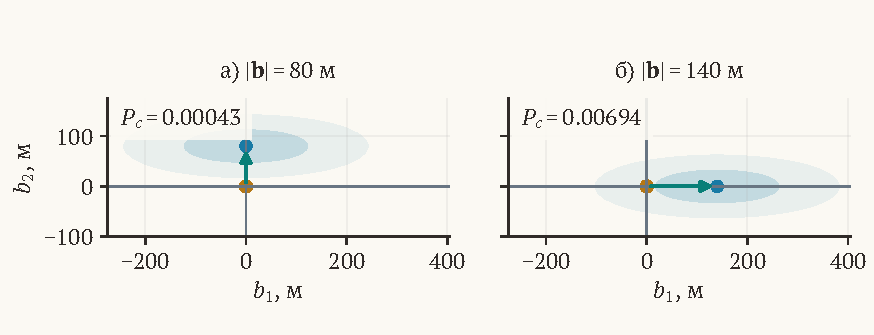
\includegraphics[width=\textwidth,height=43mm,keepaspectratio]{images/concept-risk-slide.pdf}
\par
{\eqcompact\derivationmathspacing
\[
\sigma_1=120~\text{м},\quad\sigma_2=30~\text{м},\quad R_c=10~\text{м}.
\]
}
\figcaption{Эллипсы соответствуют $k=1,2$; оранжевый круг --- область столкновения.
Больший промах может располагаться в области большей плотности.}
\end{frame}

\begin{frame}{Нулевой номинальный промах}
\relax\derivationmathspacing
\begin{columns}[T,onlytextwidth]
\begin{column}{.48\textwidth}
\textbf{Изотропная ковариация}
{\eqcompact\derivationmathspacing
\[
\vect b=0,\qquad C_b=\sigma^2I_2,
\]
\[
\begin{aligned}
P_c&=\int_0^{R_c}\frac{r}{\sigma^2}
e^{-r^2/(2\sigma^2)}\,\dd r\\
&=\boxed{1-\exp\!\left(-\frac{R_c^2}{2\sigma^2}\right).}
\end{aligned}
\]
}
При увеличении $\sigma$ вероятность убывает от единицы к нулю,
хотя номинальные траектории пересекаются.
\end{column}
\begin{column}{.49\textwidth}
\textbf{Причина уменьшения $P_c$}
\par\smallskip
Манёвр может удалить средний вектор промаха от области столкновения
при той же ковариации.
\par\smallskip
Рост неопределённости также распределяет вероятность по большей области:
в небольшой круг попадает меньшая её доля.
\par\smallskip
При ненулевом промахе зависимость от $\sigma$ может быть немонотонной.
\end{column}
\end{columns}
\end{frame}

\begin{frame}{Размывание вероятности}
\relax\derivationmathspacing
\centering
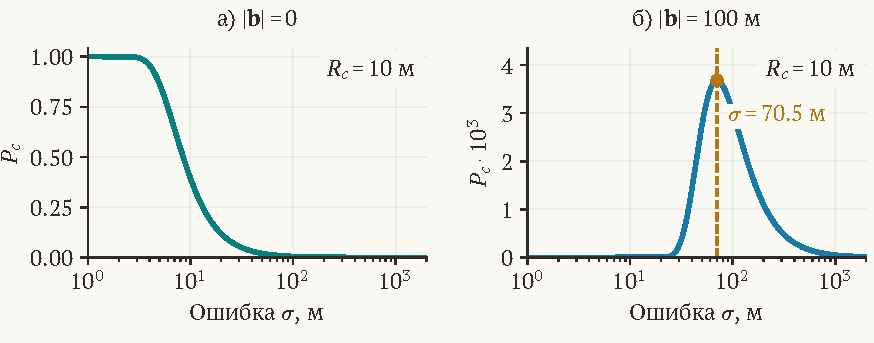
\includegraphics[width=\textwidth,height=42mm,keepaspectratio]{images/concept-dilution-slide.pdf}
\par
\figcaption{$C_b=\sigma^2I_2$, $R_c=10$~м. При промахе 100~м максимум
$P_c\approx3{,}68\cdot10^{-3}$ достигается около $\sigma=70{,}5$~м.}
\par\smallskip
\raggedright
Малое $P_c$ при большой неопределённости не означает точного прогноза большого расстояния.
Для решения оценивают достоверность ковариаций и возможность уточнить орбиты.
\end{frame}
% Главы 4--5 collision-avoidance.tex: обозначения и выводы сохранены.
\begin{frame}{Импульсный манёвр}
\relax\derivationmathspacing
{\eqcompact\derivationmathspacing
\[
 \vect e_r=\frac{\vect R_{\mathrm{sc}}}{R_{\mathrm{sc}}},\qquad
 \vect e_n=\frac{\vect R_{\mathrm{sc}}\times\vect V_{\mathrm{sc}}}
 {\norm{\vect R_{\mathrm{sc}}\times\vect V_{\mathrm{sc}}}},\qquad
 \vect e_t=\vect e_n\times\vect e_r,\qquad
 Q=[\vect e_r\ \vect e_t\ \vect e_n].
\]
}
\begin{columns}[T,onlytextwidth]
\begin{column}{.47\textwidth}
\textbf{Точный скачок скорости}
{\eqcompact\derivationmathspacing
\[
 \begin{aligned}
 \vect R_{\mathrm{sc}}^+&=\vect R_{\mathrm{sc}}^-,\\
 \vect V_{\mathrm{sc}}^+&=\vect V_{\mathrm{sc}}^-+Q\Delta\vect V,\\
 \Delta\vect V&=(\Delta V_r,\Delta V_t,\Delta V_n)^\top.
 \end{aligned}
\]
}
В момент $t_m$ положение непрерывно. Новые элементы вычисляются по прежнему положению и новой скорости.
\end{column}
\begin{column}{.50\textwidth}
\textbf{Первый порядок по импульсу}
{\eqcompact\derivationmathspacing
\[
 \delta\vect y(t_m^+)=B(\vect y_{\mathrm{sc}}(t_m))\Delta\vect V,
\]
\[
 B=\left.\frac{\partial\vect y(\vect R_{\mathrm{sc}},\vect V_{\mathrm{sc}}+Q\Delta\vect V)}
 {\partial\Delta\vect V}\right|_{\Delta\vect V=0}.
\]
}
$\vect y=(a,e,\omega,i,\Omega,M)^\top$.
\par\smallskip
$B$ совпадает с матрицей коэффициентов при ускорениях в уравнениях Гаусса.
\end{column}
\end{columns}
\end{frame}

\begin{frame}{Матрица манёвра}
\relax\derivationmathspacing
\begin{columns}[T,onlytextwidth]
\begin{column}{.48\textwidth}
\textbf{Перенос изменения элементов}
{\eqcompact\derivationmathspacing
\[
 \delta\vect y(t_{\mathrm{ca}})
 =\Phi(t_{\mathrm{ca}},t_m)\delta\vect y(t_m^+),
\]
\[
 \delta\vect y(t_{\mathrm{ca}})=M(t_m)\Delta\vect V,
\]
\[
 \boxed{M(t_m)=\Phi(t_{\mathrm{ca}},t_m)B(\vect y_{\mathrm{sc}}(t_m)).}
\]
}
В каждой эпохе номинальное и изменённое состояния сравниваются при одном физическом времени.
\end{column}
\begin{column}{.49\textwidth}
\textbf{Изменение положения}
{\eqcompact\derivationmathspacing
\[
 \boxed{\delta\vect R_{\mathrm{sc}}(t_{\mathrm{ca}})
 =\frac{\partial\vect R_{\mathrm{sc}}}{\partial\vect y_{\mathrm{sc}}}
 M(t_m)\Delta\vect V.}
\]
}
Производная берётся в $t_{\mathrm{ca}}$; перенос по времени уже учтён в $M$.
\par\smallskip
Изменение большой полуоси меняет среднее движение. Различие фаз накапливается: заблаговременный импульс может дать заметное смещение к сближению.
\end{column}
\end{columns}
\smallskip
Матрицы вычисляются вдоль номинальной траектории управляемого КА. Опасный объект прогнозируется отдельно.
\end{frame}

\begin{frame}{Смещение в плоскости сближения}
\relax\derivationmathspacing
\begin{columns}[T,onlytextwidth]
\begin{column}{.46\textwidth}
\textbf{Изменение относительного положения}
{\eqcompact\derivationmathspacing
\[
 \vect\rho=\vect R_{\mathrm{obj}}-\vect R_{\mathrm{sc}},
 \qquad\vect b=P\vect\rho,
\]
\[
 \delta\vect\rho=-\delta\vect R_{\mathrm{sc}},
\]
\[
 \delta\vect b=-P\frac{\partial\vect R_{\mathrm{sc}}}
 {\partial\vect y_{\mathrm{sc}}}M(t_m)\Delta\vect V.
\]
}
Знак минус связан с определением $\vect\rho$: маневрирует объект $\mathrm{sc}$.
\end{column}
\begin{column}{.51\textwidth}
\textbf{Линейная модель промаха}
{\eqcompact\derivationmathspacing
\[
 \boxed{\vect b\simeq\vect b_0+G(t_m)\Delta\vect V,}
\]
\[
 \boxed{G(t_m)=-P\frac{\partial\vect R_{\mathrm{sc}}}
 {\partial\vect y_{\mathrm{sc}}}M(t_m).}
\]
}
\begin{itemize}
\setlength{\itemsep}{2pt}
\item $G\in\mathbb R^{2\times3}$.
\item Столбцы соответствуют радиальной, трансверсальной и нормальной компонентам.
\item При метрах и м/с элементы $G$ имеют размерность секунды.
\end{itemize}
\end{column}
\end{columns}
\smallskip
Плоскость и эпоха номинального сближения при построении $G$ фиксированы.
\end{frame}

\begin{frame}{Вычисление матрицы $G$}
\relax\derivationmathspacing
{\eqcompact\derivationmathspacing
\[
 \boxed{G_{:,j}\simeq
 \frac{\vect b(+\varepsilon\vect d_j)
       -\vect b(-\varepsilon\vect d_j)}{2\varepsilon}.}
\]
}
\begin{columns}[T,onlytextwidth]
\begin{column}{.48\textwidth}
\textbf{Центральные конечные разности}
\begin{enumerate}
\setlength{\itemsep}{3pt}
\item Выбрать ось ОСК $\vect d_j$ и малое приращение скорости $\varepsilon$.
\item Выполнить прогнозы с импульсами $+\varepsilon\vect d_j$ и $-\varepsilon\vect d_j$.
\item Разность промахов разделить на $2\varepsilon$.
\end{enumerate}
\end{column}
\begin{column}{.49\textwidth}
\textbf{Условия сравнения}
\begin{itemize}
\setlength{\itemsep}{3pt}
\item Каждый прогноз использует точный скачок скорости.
\item В обоих прогнозах одинаковы $P$ и $t_{\mathrm{ca}}$.
\item Перенос можно вычислять с принятой моделью возмущений.
\end{itemize}
\end{column}
\end{columns}
\smallskip
Линеаризуется отклонение КА от собственной номинальной траектории.
\end{frame}

\begin{frame}{Изменение времени сближения}
\relax\derivationmathspacing
$t_0=t_{\mathrm{ca}}$ --- номинальная TCA, $t_0+\delta t$ --- новая. Индекс $\mathrm{new}$ обозначает движение после манёвра.
{\eqcompact\derivationmathspacing
\[
 \delta\vect\rho=\vect\rho_{\mathrm{new}}(t_0)-\vect\rho(t_0),\qquad
 \delta\vect v=\vect v_{\mathrm{rel,new}}(t_0)-\vect v_{\mathrm{rel}}(t_0).
\]
\[
 \begin{aligned}
 \vect\rho_{\mathrm{new}}(t_0+\delta t)-\vect\rho(t_0)
 ={}&\underbrace{\vect\rho_{\mathrm{new}}(t_0)-\vect\rho(t_0)}
 _{\delta\vect\rho:\ \text{две траектории, одно время}}\\[4mm]
 &+\underbrace{\vect\rho_{\mathrm{new}}(t_0+\delta t)
              -\vect\rho_{\mathrm{new}}(t_0)}
 _{\text{одна новая траектория, два времени}}.
 \end{aligned}
\]
}
\smallskip
Импульс не меняет положение в $t_m$. К более позднему $t_0$ движение по изменённой орбите уже может дать $\delta\vect\rho\ne0$.
\par\smallskip
$\delta\vect\rho$ ещё не учитывает переход к новому моменту события.
\end{frame}

\begin{frame}{Сдвиг момента сближения}
\relax\derivationmathspacing
Обозначим $\vect v=\vect v_{\mathrm{rel}}(t_0)$,
$\vect a=\vect a_{\mathrm{rel}}(t_0)$.
\par\smallskip
\begin{columns}[T,onlytextwidth]
\begin{column}{.47\textwidth}
\textbf{Первый порядок}
{\eqcompact\derivationmathspacing
\[
 \begin{aligned}
 \vect\rho_{\mathrm{new}}(t_0+\delta t)
   &\simeq\vect\rho(t_0)+\delta\vect\rho+\vect v\delta t,\\
 \vect v_{\mathrm{rel,new}}(t_0+\delta t)
   &\simeq\vect v+\delta\vect v+\vect a\delta t.
 \end{aligned}
\]
}
Произведение $\delta\vect v\,\delta t$ имеет второй порядок по малому манёвру.
\end{column}
\begin{column}{.50\textwidth}
\textbf{Условие нового минимума}
{\eqcompact\derivationmathspacing
\[
 \vect\rho_{\mathrm{new}}\cdot\vect v_{\mathrm{rel,new}}=0,
 \qquad\vect\rho(t_0)\cdot\vect v=0,
\]
\[
 \begin{aligned}
 &\vect v\cdot\delta\vect\rho+\vect\rho(t_0)\cdot\delta\vect v\\
 &\quad+\bigl(\norm{\vect v}^2+\vect\rho(t_0)\cdot\vect a\bigr)\delta t\simeq0.
 \end{aligned}
\]
}
\end{column}
\end{columns}
{\eqcompact\derivationmathspacing
\[
 \boxed{\delta t=-\frac{\vect v\cdot\delta\vect\rho
          +\vect\rho(t_0)\cdot\delta\vect v}
          {\norm{\vect v}^2+\vect\rho(t_0)\cdot\vect a}.}
\]
}
Знаменатель положителен для невырожденного минимума.
$P\vect v\delta t=0$: сдвиг времени не меняет проекцию в первом порядке.
Итоговый прогноз заново определяет TCA и плоскость.
\end{frame}

\begin{frame}{Манёвр заданного направления}
\relax\derivationmathspacing
{\eqcompact\derivationmathspacing
\[
 \Delta\vect V=s\vect d,\quad s\geqslant0,\quad\norm{\vect d}=1,
 \qquad \vect b(s)=\vect b_0+sG(t_m)\vect d.
\]
}
\centering
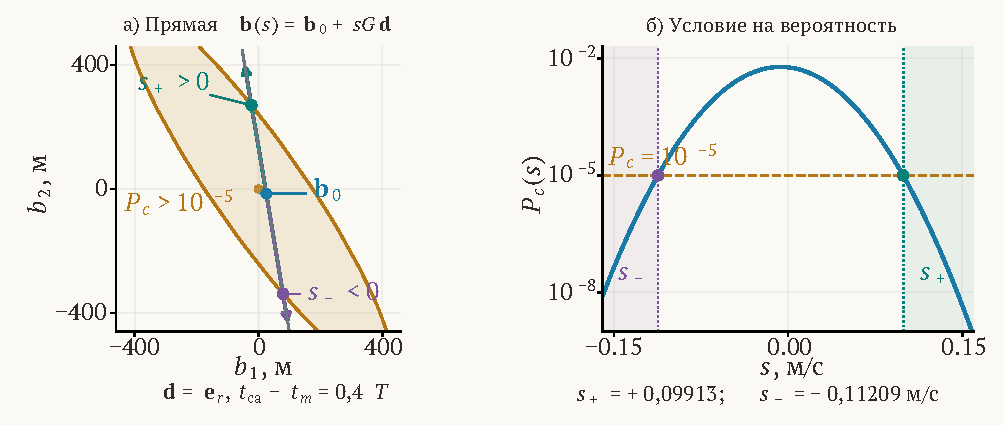
\includegraphics[width=\textwidth,height=43mm,keepaspectratio]{images/design-fixed-direction-slide.pdf}\par
\raggedright
\figcaption{Проверяются оба знака импульса. Переходы через $P_{\text{доп}}$ уточняются одномерным поиском корня; выбирается ближайшая допустимая граница.}
\end{frame}

\begin{frame}{Наибольший промах}
\relax\derivationmathspacing
При заданных $t_m$ и $d$ сначала примем $\vect b_0=0$.
\begin{columns}[T,onlytextwidth]
\begin{column}{.47\textwidth}
\textbf{Геометрическая задача}
{\eqcompact\derivationmathspacing
\[
 \vect b=G\Delta\vect V,
\]
\[
 \norm{\vect b}^2=\Delta\vect V^\top G^\top G\Delta\vect V,
\]
\[
 \begin{aligned}
 \max_{\Delta\vect V}\quad&\norm{\vect b}^2,\\[2pt]
 \mathrm{s.t.}\quad&\vect b=G\Delta\vect V,\\
 &\norm{\Delta\vect V}=d.
 \end{aligned}
\]
}
\end{column}
\begin{column}{.50\textwidth}
\textbf{Собственный базис $G^\top G$}
\par\smallskip
Матрица симметрична и неотрицательно определена. $\alpha_j$ --- компоненты импульса в её собственном базисе.
{\eqcompact\derivationmathspacing
\[
 \begin{aligned}
 \norm{\vect b}^2&=\sum_j\lambda_j\alpha_j^2\\
 &\leqslant\lambda_{\max}\sum_j\alpha_j^2
 =\lambda_{\max}d^2.
 \end{aligned}
\]
}
Равенство достигается, если импульс направлен вдоль собственного вектора с наибольшим собственным значением.
\end{column}
\end{columns}
\end{frame}

\begin{frame}{Отображение импульсов в промахи}
\relax\derivationmathspacing
\centering
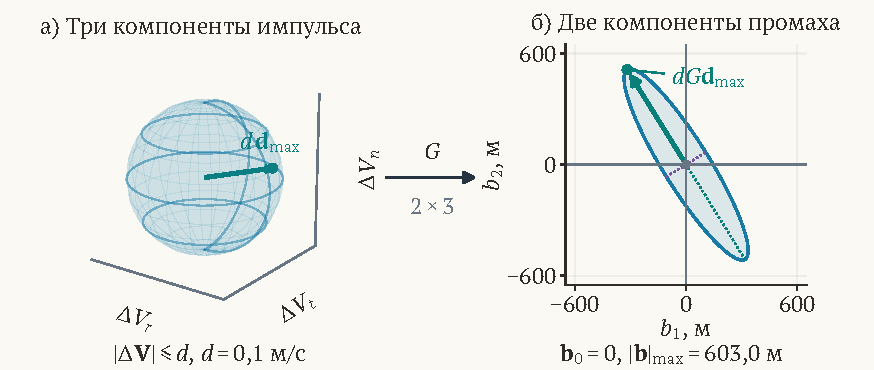
\includegraphics[width=\textwidth,height=45mm,keepaspectratio]{images/design-impulse-map-slide.pdf}\par
{\eqcompact\derivationmathspacing
\[
 \Delta\vect V=\pm d\vect d_{\max},\quad
 G^\top G\vect d_{\max}=\lambda_{\max}\vect d_{\max},\quad
 b_{\max}=d\sqrt{\lambda_{\max}}.
\]
}
\raggedright
\figcaption{При $\vect b_0=0$ шар допустимых импульсов отображается в заполненный эллипс. Его большая полуось задаёт наибольший промах.}
\end{frame}

\begin{frame}{Ненулевой исходный промах}
\relax\derivationmathspacing
\begin{columns}[T,onlytextwidth]
\begin{column}{.44\textwidth}
\textbf{Полная постановка}
{\eqcompact\derivationmathspacing
\[
 \begin{aligned}
 \max_{\Delta\vect V}\quad&\norm{\vect b_0+G\Delta\vect V}^2,\\[3pt]
 \mathrm{s.t.}\quad&\norm{\Delta\vect V}=d.
 \end{aligned}
\]
}
$t_m$ и величина импульса $d$ фиксированы.
\par\smallskip
Направление выбирается с учётом уже имеющегося $\vect b_0$.
\end{column}
\begin{column}{.53\textwidth}
\textbf{Разложение критерия}
{\eqcompact\derivationmathspacing
\[
 \begin{aligned}
 \norm{\vect b_0+G\Delta\vect V}^2
 ={}&\norm{\vect b_0}^2\\
 &+2\Delta\vect V^\top G^\top\vect b_0\\
 &+\Delta\vect V^\top G^\top G\Delta\vect V.
 \end{aligned}
\]
}
Появляется линейный член: противоположные импульсы не равноценны.
\par\smallskip
Главный собственный вектор в общем случае не решает эту задачу. В примере направление уточняется численно на сфере.
\end{column}
\end{columns}
\end{frame}

\begin{frame}{Расстояние Махаланобиса}
\relax\derivationmathspacing
{\eqcompact\derivationmathspacing
\[
 D^2=\vect b^\top C_b^{-1}\vect b
    =\frac{\beta_1^2}{\sigma_1^2}+\frac{\beta_2^2}{\sigma_2^2}.
\]
}
\centering
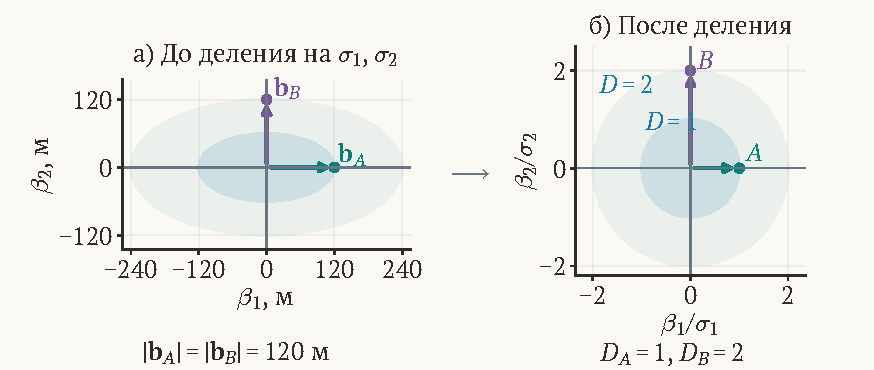
\includegraphics[width=\textwidth,height=40mm,keepaspectratio]{images/design-mahalanobis-slide.pdf}\par
\raggedright
\figcaption{$\beta_1,\beta_2$ --- компоненты в главных осях ковариации. После деления на $\sigma_1,\sigma_2$ длина вектора равна $D$. Одинаковые промахи могут давать разные $D$.}
\end{frame}

\begin{frame}{Приближение вероятности}
\relax\derivationmathspacing
\textbf{Плотность из интеграла вероятности}
{\eqcompact\derivationmathspacing
\[
 f(\vect z)=\frac{1}{2\pi\sqrt{\det C_b}}
 \exp\left[-\frac12(\vect z-\vect b)^\top C_b^{-1}(\vect z-\vect b)\right],
 \qquad
 P_c=\iint_{\norm{\vect z}\leqslant R_c}f(\vect z)\,\dd z_1\dd z_2.
\]
}
\begin{columns}[T,onlytextwidth]
\begin{column}{.48\textwidth}
\textbf{Почти постоянная плотность в круге}
{\eqcompact\derivationmathspacing
\[
 \boxed{P_c\simeq\pi R_c^2 f(0)
 =\frac{R_c^2}{2\sqrt{\det C_b}}e^{-D^2/2}.}
\]
}
Площадь области столкновения умножается на плотность в её центре.
\par\smallskip
При фиксированных $C_b,R_c$ увеличение $D^2$ приближённо уменьшает $P_c$.
\end{column}
\begin{column}{.49\textwidth}
\textbf{Выбор направления при $\vect b_0=0$}
{\eqcompact\derivationmathspacing
\[
 D^2=\Delta\vect V^\top G^\top C_b^{-1}G\Delta\vect V.
\]
}
В собственной задаче вместо $G^\top G$ используется $G^\top C_b^{-1}G$.
\par\smallskip
Направления обычно различаются. Точный интеграл в общем случае не определяется одним $D^2$.
\end{column}
\end{columns}
\end{frame}

\begin{frame}{Изменение плотности}
\relax\derivationmathspacing
Деление $f(\vect z)$ на $f(0)$ сокращает нормирующий множитель.
{\eqcompact\derivationmathspacing
\[
 \begin{aligned}
 \log\frac{f(\vect z)}{f(0)}
 &=-\frac12\left[(\vect z-\vect b)^\top C_b^{-1}(\vect z-\vect b)
                         -\vect b^\top C_b^{-1}\vect b\right]\\
 &=\vect z^\top C_b^{-1}\vect b-\frac12\vect z^\top C_b^{-1}\vect z.
 \end{aligned}
\]
}
\begin{columns}[T,onlytextwidth]
\begin{column}{.48\textwidth}
\textbf{Линейный член при $\norm{\vect z}\leqslant R_c$}
{\eqcompact\derivationmathspacing
\[
 |\vect z^\top C_b^{-1}\vect b|
 \leqslant R_c\norm{C_b^{-1}\vect b}.
\]
}
При большом удалении среднего вектора промаха этот член может быть существенным.
\end{column}
\begin{column}{.49\textwidth}
\textbf{Квадратичный член}
{\eqcompact\derivationmathspacing
\[
 \tfrac12|\vect z^\top C_b^{-1}\vect z|
 \leqslant\tfrac12R_c^2\lambda_{\max}(C_b^{-1}).
\]
}
Для почти постоянной плотности обе оценки должны быть малы.
\end{column}
\end{columns}
\smallskip
Одного условия $R_c\ll\sigma_{\min}$ недостаточно. Приближённое направление проверяют непосредственным вычислением $P_c$.
\end{frame}

\begin{frame}{Минимальная характеристическая скорость}
\relax\derivationmathspacing
\begin{columns}[T,onlytextwidth]
\begin{column}{.58\textwidth}
\textbf{Фиксированное время $t_m$}
{\eqcompact\derivationmathspacing
\[
 \begin{aligned}
 \min_{\mathclap{\Delta\vect V\in\mathcal A(t_m)}}\quad
  &\norm{\Delta\vect V},\\[4pt]
 \mathrm{s.t.}\quad
  &P_c(\vect b_0+G(t_m)\Delta\vect V,C_b,R_c)
  \leqslant P_{\text{доп}}.
 \end{aligned}
\]
}
$C_b$ --- номинальная ковариация; $\mathcal A$ ограничивает направление и величину импульса.
\par\smallskip
При свободном времени повторяют поиск по допустимым $t_m$ или оптимизируют время вместе с импульсом.
\end{column}
\begin{column}{.39\textwidth}
\textbf{Численное уточнение}
\begin{enumerate}
\setlength{\itemsep}{3pt}
\item Найти допустимые варианты одномерным поиском.
\item Уточнить три компоненты.
\item Сравнить несколько начальных приближений.
\item Проверить исходной моделью.
\end{enumerate}
\end{column}
\end{columns}
\smallskip
Область безопасности не выпукла. Несколько начальных приближений уменьшают зависимость от локального решения, но не доказывают глобальный минимум.
\end{frame}
% Главы 6--7 действующей методички collision-avoidance.tex.
% Численные данные, критерии и обозначения сохранены.

\begin{frame}{Пространственное сближение}
\relax\derivationmathspacing
\begin{columns}[T,onlytextwidth]
\begin{column}{.48\textwidth}
\textbf{Управляемый аппарат в TCA}
{\eqcompact\derivationmathspacing
\[
\begin{aligned}
 a_{\mathrm{sc}}&=7000\ \text{км},& e_{\mathrm{sc}}&=0{,}01,\\
 \omega_{\mathrm{sc}}&=40^\circ,& i_{\mathrm{sc}}&=51^\circ,\\
 \Omega_{\mathrm{sc}}&=20^\circ,& \nu_{\mathrm{sc}}&=60^\circ.
\end{aligned}
\]
\[
 \mu=398600{,}4418\ \text{км}^3/\text{с}^2,
 \qquad T=\ExamplePeriod\ \text{с}.
\]
}
Центральное поле Земли; номинальная TCA задаёт $t=0$.
\par\smallskip
Синтетический пример позволяет сопоставить геометрический и вероятностный критерии.
\end{column}
\begin{column}{.49\textwidth}
\centering
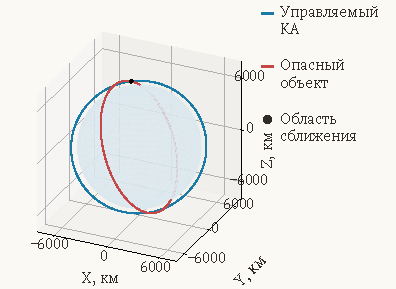
\includegraphics[width=67mm,height=49mm,keepaspectratio]{images/example-orbits-slide.pdf}
\par\smallskip
\raggedright Разные плоскости орбит; промах $\ExampleNominalMiss$~м в этом масштабе неразличим.
\end{column}
\end{columns}
\end{frame}

\begin{frame}{Состояние опасного объекта}
\relax\derivationmathspacing
В эпоху $t=0$ радиальную компоненту скорости сохраним, трансверсальную повернём на $60^\circ$.
\begin{columns}[T,onlytextwidth]
\begin{column}{.48\textwidth}
{\eqcompact\derivationmathspacing
\[
\begin{aligned}
 \vect V_{\mathrm{obj}}={}&V_{r,\mathrm{sc}}\vect e_{r,\mathrm{sc}}\\
 &+V_{t,\mathrm{sc}}\cos60^\circ\,\vect e_{t,\mathrm{sc}}\\
 &+V_{t,\mathrm{sc}}\sin60^\circ\,\vect e_{n,\mathrm{sc}}.
\end{aligned}
\]
\[
 \vect e_1=\vect e_{r,\mathrm{sc}},\qquad
 \vect e_2=\vect e_v\times\vect e_1,
\]
\[
 \vect b_0=\begin{pmatrix}25\\-15\end{pmatrix}\text{м},\qquad
 \vect R_{\mathrm{obj}}=\vect R_{\mathrm{sc}}+P^\top\vect b_0.
\]
}
Положения и промах предварительно выражаются в одних единицах.
\end{column}
\begin{column}{.49\textwidth}
\textbf{Полученная эллиптическая орбита}
{\eqcompact\derivationmathspacing
\[
\begin{aligned}
 a_{\mathrm{obj}}&\approx7000{,}050512\ \text{км},\\
 e_{\mathrm{obj}}&\approx0{,}0100002244,\\
 i_{\mathrm{obj}}&\approx64{,}43534^\circ,\\
 \Omega_{\mathrm{obj}}&\approx90{,}98391^\circ,\\
 \omega_{\mathrm{obj}}&\approx-1{,}93879^\circ.
\end{aligned}
\]
\[
 \begin{aligned}
 \vect\rho\cdot\vect v_{\mathrm{rel}}&=0,\\
 \norm{\vect v_{\mathrm{rel}}}&=\ExampleRelativeSpeed\ \text{км/с}.
 \end{aligned}
\]
}
В $t=0$ проверен локальный минимум расстояния.
\end{column}
\end{columns}
\end{frame}

\begin{frame}{Неопределённость расчётного сближения}
\relax\derivationmathspacing
\begin{columns}[T,onlytextwidth]
\begin{column}{.48\textwidth}
\textbf{Ковариация в эпоху TCA}
{\eqcompact\derivationmathspacing
\[
 C_b=\begin{pmatrix}
 14233{,}213&-18042{,}098\\
 -18042{,}098&27366{,}787
 \end{pmatrix}\text{м}^2.
\]
\[
 \sigma_1=40\ \text{м},\qquad \sigma_2=200\ \text{м}.
\]
}
Ось ошибки $40$~м повёрнута на $35^\circ$ от $b_1$ к $b_2$.
{\eqcompact\derivationmathspacing
\[
 C_\rho=P^\top C_bP+(300\ \text{м})^2\vect e_v\vect e_v^\top.
\]
}
В короткой окрестности события $C_\rho$ постоянна в инерциальных осях.
\end{column}
\begin{column}{.49\textwidth}
\textbf{Исходная опасность}
\[
 R_c=10\ \text{м},\qquad P_{\text{доп}}=10^{-5},
\]
\[
 \boxed{P_{c,0}=\ExampleNominalPc>10^{-5}.}
\]
\begin{itemize}
\setlength{\itemsep}{4pt}
\item Продольный размер $3\sigma=900$~м проходится примерно за $0{,}12$~с.
\item Краткость пролёта согласуется с двумерной моделью.
\item Ковариация задана как условие учебной задачи непосредственно в TCA.
\end{itemize}
\end{column}
\end{columns}
\end{frame}

\begin{frame}{Матрица влияния импульса}
\relax\derivationmathspacing
Основной момент манёвра: $t_m=-0{,}4T=-\ExampleLead$~с.
{\eqcompact\derivationmathspacing
\[
 \vect b\simeq\vect b_0+G\Delta\vect V,\qquad
 G=\begin{pmatrix}
 -483{,}069&-3321{,}815&0\\
 2882{,}996&4276{,}692&-256{,}984
 \end{pmatrix}\text{с}.
\]
}
\begin{columns}[T,onlytextwidth]
\begin{column}{.48\textwidth}
\textbf{Расчёт чувствительности}
\begin{itemize}
\setlength{\itemsep}{4pt}
\item Центральные конечные разности по компонентам импульса.
\item Шаг $0{,}001$~м/с; компоненты заданы в текущей ОСК управляемого КА.
\end{itemize}
\end{column}
\begin{column}{.49\textwidth}
\textbf{Геометрический смысл}
\begin{itemize}
\setlength{\itemsep}{4pt}
\item Два компонента промаха получают вклады от трёх компонентов импульса.
\item Практически нулевой элемент нормального столбца в первой строке связан с выбранной геометрией.
\end{itemize}
\end{column}
\end{columns}
\end{frame}

\begin{frame}{Ограничение направления манёвра}
\relax\derivationmathspacing
Для каждого направления ОСК проверяются оба знака и выбирается наименьший по модулю импульс при $P_c=10^{-5}$.
\par\smallskip
\centering
{\eqcompact
\renewcommand{\arraystretch}{1.2}
\begin{tabular}{@{}lrr@{}}
\toprule
Направление & Компонента импульса, м/с & Промах $\norm{\vect b}$, м\\\midrule
Радиальное & $0{,}099133$ & $271{,}77$\\
Трансверсальное & $-0{,}121313$ & $684{,}20$\\
Нормальное & $-0{,}876068$ & $211{,}62$\\
\bottomrule
\end{tabular}\par
}
\raggedright\medskip
\begin{columns}[T,onlytextwidth]
\begin{column}{.48\textwidth}
\begin{block}{Один уровень вероятности}
Различные нормы промаха на границе $P_c=10^{-5}$ отражают анизотропию ковариации.
\end{block}
\end{column}
\begin{column}{.49\textwidth}
\begin{block}{Различная цена направления}
Нормальный манёвр в выбранную эпоху значительно менее эффективен, чем радиальный и трансверсальный.
\end{block}
\end{column}
\end{columns}
\end{frame}

\begin{frame}{Два критерия выбора манёвра}
\relax\derivationmathspacing
\begin{columns}[T,onlytextwidth]
\begin{column}{.46\textwidth}
\textbf{Максимальный промах}
{\eqcompact\derivationmathspacing
\[
 \begin{aligned}
 J&=0{,}1\ \text{м/с},\quad \norm{\vect b}=629{,}11\ \text{м},\\
 P_c&=3{,}90\cdot10^{-5}>P_{\text{доп}}.
 \end{aligned}
\]
}
\textbf{Минимальный импульс}
{\eqcompact\derivationmathspacing
\[
 \Delta\vect V\approx
 \begin{pmatrix}0{,}095635\\0{,}017739\\-0{,}010576\end{pmatrix}\text{м/с},
\]
\[
 \begin{aligned}
 J&=\ExampleOptimalDV\ \text{м/с},\\
 \norm{\vect b}&=348{,}63\ \text{м},\qquad P_c=10^{-5}.
 \end{aligned}
\]
}
\figcaption{Лучший найденный вариант при $t_m=-0{,}4T$; глобальный минимум не доказан.
Линии --- уровни $P_c$; пунктир --- $\vect b^\top C_b^{-1}\vect b=1$.}
\end{column}
\begin{column}{.53\textwidth}
\centering
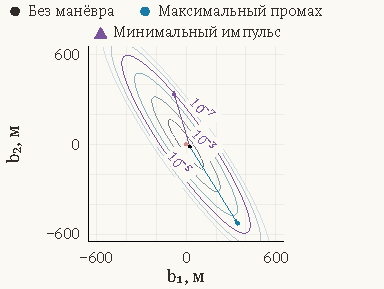
\includegraphics[width=\linewidth,height=60mm,keepaspectratio]{images/example-bplane-slide.pdf}
\end{column}
\end{columns}
\end{frame}

\begin{frame}{Промах и время упреждения}
\relax\derivationmathspacing
\centering
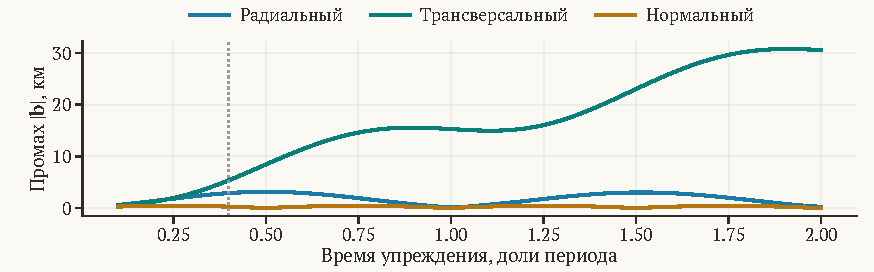
\includegraphics[width=\textwidth,height=46mm,keepaspectratio]{images/example-lead-top-slide.pdf}
\par\smallskip\raggedright
\begin{columns}[T,onlytextwidth]
\begin{column}{.48\textwidth}
Показан $\norm{\vect b}$ при импульсе $+1$~м/с вдоль каждого направления ОСК.
\end{column}
\begin{column}{.49\textwidth}
Для каждого $t_m$ заново вычисляются текущая ОСК и $G$; ковариация в TCA фиксирована.
\end{column}
\end{columns}
\end{frame}

\begin{frame}{Импульс и время упреждения}
\relax\derivationmathspacing
\centering
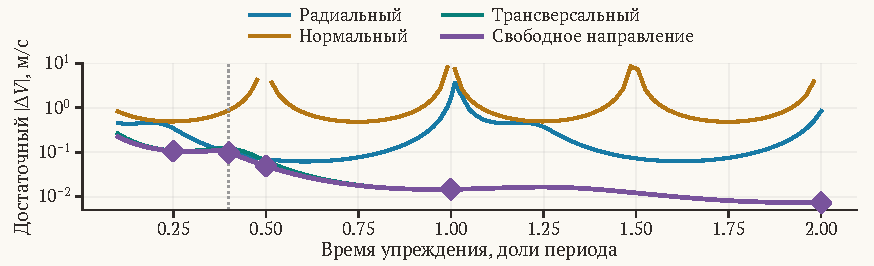
\includegraphics[width=\textwidth,height=45mm,keepaspectratio]{images/example-lead-bottom-slide.pdf}
\par\smallskip\raggedright
\begin{columns}[T,onlytextwidth]
\begin{column}{.48\textwidth}
Свободное направление: $0{,}10605$~м/с за $0{,}25T$ и $0{,}04895$~м/с за $0{,}5T$.
\end{column}
\begin{column}{.49\textwidth}
За $T$ --- $0{,}01453$~м/с; за $2T$ --- $0{,}007265$~м/с. Накапливается фазовый сдвиг.
\end{column}
\end{columns}
\end{frame}

\begin{frame}{Выбор трансверсального импульса}
\relax\derivationmathspacing
\begin{columns}[T,onlytextwidth]
\begin{column}{.61\textwidth}
\centering
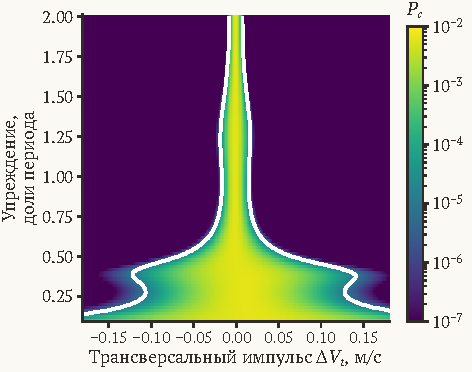
\includegraphics[width=\linewidth,height=62mm,keepaspectratio]{images/example-risk-map-slide.pdf}
\end{column}
\begin{column}{.36\textwidth}
Контур $P_c=10^{-5}$ отделяет допустимые варианты линейной модели.
\par\smallskip
Тепловая карта связывает знак и величину импульса с временем упреждения.
\end{column}
\end{columns}
\end{frame}

\begin{frame}{Нелинейная проверка манёвра}
\relax\derivationmathspacing
\begin{columns}[T,onlytextwidth]
\begin{column}{.48\textwidth}
После точного скачка скорости восстанавливаются элементы; обе орбиты прогнозируются в классических элементах через уравнение Кеплера.
{\eqcompact\derivationmathspacing
\[
 \begin{aligned}
 \vect\rho\cdot\vect v_{\mathrm{rel}}&=0,\\
 \Delta t_{\mathrm{TCA}}&=\ExampleOptimalTCA\ \text{с}.
 \end{aligned}
\]
\[
\begin{aligned}
 \text{Линейно: }\norm{\vect b}&=\ExampleOptimalMiss\ \text{м},\\
 \text{Повтор: }d_{\min}&=\ExampleOptimalNonlinearMiss\ \text{м},\\
 P_c&\approx9{,}9992\cdot10^{-6}.
\end{aligned}
\]
}
В новой TCA заново строится плоскость и проектируется $C_\rho$. Запас по вероятности практически отсутствует.
\end{column}
\begin{column}{.49\textwidth}
\centering
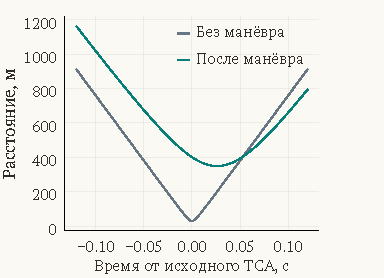
\includegraphics[width=65mm,height=47mm,keepaspectratio]{images/example-local-distance-slide.pdf}
\par\smallskip
\raggedright Большая относительная скорость быстро увеличивает расстояние вне минимума.
\end{column}
\end{columns}
\end{frame}

\begin{frame}{Ошибки исполнения импульса}
\relax\derivationmathspacing
\begin{columns}[T,onlytextwidth]
\begin{column}{.48\textwidth}
\textbf{Линейный перенос ошибки}
\par\smallskip
Фактически выполнен импульс $\Delta\vect V+\vect\varepsilon_V$.
{\eqcompact\derivationmathspacing
\[
 \mathbb E\,\vect\varepsilon_V=0,\qquad
 \text{ошибка промаха: }G\vect\varepsilon_V,
\]
\[
 \boxed{C_{b,\mathrm{tot}}=C_b+G C_{\Delta V}G^\top.}
\]
}
Ошибки импульса независимы от исходных ошибок состояния. Добавляется неопределённость, ещё не учтённая в $C_b$.
\end{column}
\begin{column}{.49\textwidth}
\textbf{Принятая абсолютная модель}
{\eqcompact\derivationmathspacing
\[
 C_{\Delta V}=\sigma_V^2I_3,\qquad
 \sigma_V=0{,}005\ \text{м/с},
\]
\[
 \boxed{P_c=\ExampleExecutionPc>10^{-5}.}
\]
}
Номинальный импульс на границе допустимости не оставляет запаса для этой ошибки.
\par\smallskip
Систематическая ошибка смещает ожидаемый вектор промаха; одной добавки к дисперсии недостаточно.
\end{column}
\end{columns}
\end{frame}

\begin{frame}{Манёвр с запасом по вероятности}
\relax\derivationmathspacing
\begin{columns}[T,onlytextwidth]
\begin{column}{.48\textwidth}
Повторим оптимизацию с $C_{b,\mathrm{tot}}$ и расчётным ограничением $P_c\leqslant8\cdot10^{-6}$.
{\eqcompact\derivationmathspacing
\[
 \Delta\vect V=\begin{pmatrix}
 0{,}098719\\0{,}018319\\-0{,}010917
 \end{pmatrix}\text{м/с},
\]
\[
 \boxed{J=\ExampleSafeDV\ \text{м/с}.}
\]
}
Запас выбран относительно исходного порога $10^{-5}$ для принятой модели ошибок.
\end{column}
\begin{column}{.49\textwidth}
\textbf{Повторный прогноз}
{\eqcompact\derivationmathspacing
\[
\begin{aligned}
 \Delta t_{\mathrm{TCA}}&=\ExampleSafeTCA\ \text{с},\\
 d_{\min}&=\ExampleSafeNonlinearMiss\ \text{м},\\
 P_c&\simeq\ExampleSafeNonlinearPc<10^{-5}.
\end{aligned}
\]
}
\begin{itemize}
\setlength{\itemsep}{4pt}
\item Исходная ковариация проектируется на новую плоскость.
\item Чувствительность к ошибке импульса пересчитывается около найденного управления.
\end{itemize}
\end{column}
\end{columns}
\end{frame}

\begin{frame}{Итоговая проверка манёвра}
\relax\derivationmathspacing
\begin{columns}[T,onlytextwidth]
\begin{column}{.48\textwidth}
\textbf{Траектория и исходное событие}
\begin{enumerate}
\setlength{\itemsep}{5pt}
\item Прогноз с управлением и принятой моделью возмущений.
\item Новые TCA, относительная скорость и плоскость сближения.
\item Вероятность с согласованной ковариацией и ошибками исполнения.
\end{enumerate}
\end{column}
\begin{column}{.49\textwidth}
\textbf{Ограничения и действия}
\begin{itemize}
\setlength{\itemsep}{5pt}
\item Окно подготовки, направление, ресурс ДУ и рабочая орбита.
\item Другие сближения; согласование действий активных объектов.
\item Обновление состояний и ковариаций по новым измерениям.
\item После исполнения --- прогноз от достигнутого состояния.
\end{itemize}
\end{column}
\end{columns}
\smallskip
Проверены исходная пара и принятая модель ошибок. Каталог других объектов в учебном примере не проверялся.
\end{frame}

\begin{frame}{Литература}
\relax\derivationmathspacing
\begin{enumerate}
\setlength{\itemsep}{5pt}
\item Gonzalo J.\,L., Colombo C., Di Lizia P. Analytical framework for space debris collision avoidance maneuver design. \textit{JGCD}. 2021. Vol.\,44, no.\,3. P.\,469--487.
\item NASA. \textit{Spacecraft Conjunction Assessment and Collision Avoidance Best Practices Handbook}. Rev.\,1. 2023. Приложения M--N.
\item Li J.-S., Yang Z., Luo Y.-Z. A review of space-object collision probability computation methods. \textit{Astrodynamics}. 2022. Vol.\,6, no.\,2. P.\,95--120.
\item Pavanello Z. et al. CAMmary: A Review of Spacecraft Collision Avoidance Manoeuvre Design Methods. 2025. arXiv:2503.22555.
\item NASA CARA. \textit{Step 3: Close Approach Risk Mitigation}.
\end{enumerate}
\end{frame}

\end{document}
